Прежде всего возникает вопрос: а зачем вообще нам нужны нетрадиционные методы оптимизации, раз мы уже разобрали градиентные спуски на любой вкус и цвет, методы Ньютона и прочая, и прочая, и прочая? Дело в том, что разобранные нами методы для условной оптимизации подходят не для всех множеств (например, мы можем захотеть оптимизировать функцию $f(x)$ по шару $x^T x = 1$, а метод барьеров не умеет работать с множествами без внутренности).

Рассмотрим еще один простой пример. Частая проблема в рекуррентных сетях - затухание градиента (когда норма весов $\|W\| < 1$) или взрыв градиента (соответствено, $\|W\| > 1$). Хорошей практикой здесь считается брать матрицу весов $W$ ортогональной, что позволяет контролировать ее норму (она становится единичной). Прелесть римановской оптимизации в том, что она позволяет оптимизировать функции по очень сложным множествам (типа множества ортогональных матриц или шара без внутренности).

Центральным понятием в римановской оптимизации явлется риманов градиент. Рассмотрим ради простоты всю конструкцию на сфере $S^{n-1}$. Рассмотрим некоторую точку сферы $x$ и ее окрестность. \textbf{Римановым градиентом} $\grad f(x)$ называется направление кривой наибольшего возрастания в окрестности точки $x$. Он представляет собой вектор, лежащий в касательной плоскости к сфере в точке $x$.

Казалось бы все, наши проблемы решены! Берем и делаем шаг вдоль направления риманова антиградиента. Но есть проблема: такой шаг выведет нас за пределы нашего множества:

$$
x_{k+1} = x_k - \alpha_k \grad f(x_k) \not\in S^{n-1}
$$

\noindent
Нам нужно как-то шагнуть в сторону уменьшения функции, но при этом остаться на сфере. Для этого вводится операция \textbf{ретракции} - это в некотором смысле проецирование риманова градиента на наше множества. По итогу, чтобы задать риманов градиентный спуск (RGD), нам нужно определить риманов градиент и операцию ретракцию.

$$
x_{k+1} = R_{x_k}\big(-\alpha_k \grad f(x_k)\big)
$$

\begin{figure}[H]
    \centering
    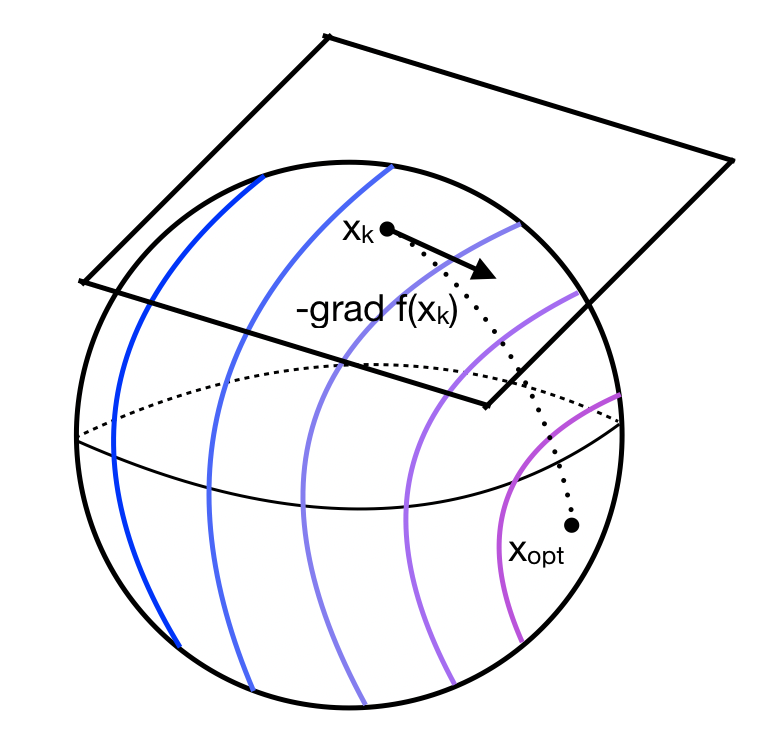
\includegraphics[width=8cm]{images/2-14-sphere.png}
    \caption{Риманов антиградиент в точке $x_k$. Цветными кривыми показаны линии уровня функции $f(x)$.}
    \label{fig:my_label}
\end{figure}

Теперь перейдем к формализму (наверное, правильнее начинать рассказывать билет отсюда, а все, что выше, приведено для понимания общей логики происходящего).

\textbf{Многообразием} $M$ размерности $d$ называется множество, удовлетворяющее двум свойствам:

\begin{enumerate}
    \item $\forall x \in M, U$ - открестность $x$ $\exists$ отображение $\phi: U \rightarrow \R^d$, биективно переводящее $U$ в некоторое открытое множество. Пара $(U, \phi)$ называется картой множества $M$.
    \item Для карт $(U, \phi), (W, \psi)$ в точке $x: U \cap W \ne \O$ отображения $\phi \circ \psi^{-1}$ и $\psi \circ \phi^{-1}$ дифференцируемы бесконечное число раз как функции $\R^d \rightarrow \R^d$.
\end{enumerate}

При этом $\phi(x) \in \R^d$ называются локальными координатами, а если $M \subset \R^n$, то $x \in \R^n$ называются глобальными координатами.

\underline{Примеры многообразий}:

\begin{enumerate}
    \item Окружность $S^1 = \{(x_1, x_2): x_1^2 + x_2^2 = 1\}$. Тогда $t \in [0, 2\pi)$ - это локальные координаты, а в качестве отображения $\phi(x)$ можно взять подходящую обратную тригонометрическую функцию.
    \item Все пространство $\R^n$. В качестве биекции берем тривиальную, а локальные координаты совпадают с глобальными.
    \item Манифолд Штифеля $\text{St}(m, n) = \{X \in \R^{n \times m} \big| X^T X = I_m\}$ (в сущности, множество ортогональных матриц).
\end{enumerate}

\textbf{Касательным пространством} в точке $x \in M$ называется множество $T_x M = \{\xi \in \R^n \big| \xi = \gamma'(0), \text{ где } \gamma(t) - \text{ это кривая в } M \text{ и } \gamma(0) = x\}$. По сути, это множество всех направлений кривых на $M$ в точке $x$.

Для примера найдем касательное пространство для шара $S^{n-1} = \{x \in \R^n \big| x^T x = 1\}$ в точке $x_0$. Интересующее нас множество кривых выглядит так:

$$
\begin{cases}
    x(t)^T x(t) = 1 \\
    x(0) = x_0
\end{cases}
$$

\noindent
Продифференцируем первое уравнение по $t$ и подставим $t=0$:

$$
x'(0)^T x(0) + x(0)^T x'(0) = 0 \Rightarrow x'(0)^T x_0 = 0
$$

\noindent
Обозначим $U_{x_0} = \{z | z^T x_0 = 0\}$. Мы только что доказали, что $T_{x_0} S^{n-1} \subseteq U_{x_0}$. Осталось показать обратное вложение. Пусть $x(t) = \frac{x_0 + tz}{\|x_0 + tz\|}$. Утверждение $x(0) = x_0$ тривиально. Нужно проверить, что $x'(0) = z$:

$$
x^i(t) = \frac{x_0^i + tz^i}{\|x_0 + tz\|}
$$

$$
x^i(t)' = \frac{z^i \|x_0 + tz\| - (x_0^i + tz^i) \frac{2\sum_{j=1}^n (x_0^j + t z^j)z^j}{2\|x_0 + tz\|}}{\|x_0 + tz\|^2} = z^i \frac{1}{\|x_0 + tz\|} - (x_0^i + tz^i) \frac{z^T (x_0 + tz)}{\|x_0 + tz\|^3}
$$

$$
x^i(0)' = z^i - x_0^i z^T x_0 = z^i
$$

\noindent
Таким образом, $x'(0) = z$, а значит, $U_{x_0} \subseteq T_{x_0} S^{n-1}$, и поэтому $T_{x_0} S^{n-1} = U_{x_0}$. Мы получили, что касательное простанство к шару - это множество векторов, перпендикулярных радиусу, что логично. Тут нужно сделать еще два важных замечания:

\begin{enumerate}
    \item $T_x M$ - линейное подпространство
    \item $\Dim T_x M = \Dim M$
\end{enumerate}

Теперь мы готовы ввести центральное понятие. \textbf{Римановым многообразием} называется многообразие $M$, снабженное скалярным произведением на каждом касательном пространстве $T_x M$, его принято обозначать $g_x(\cdot, \cdot) = \langle \cdot, \cdot \rangle_x$. Если $M \subset \R^n$, то в качестве скалярного произведение удобно брать стандартное евклидово.

\textbf{Производной по направлению} $\xi$ в римановском случае называется
$$
D f(x) [\xi] = \frac{df(\gamma(t))}{dt} \bigg|_{t = 0}, \text{ где } \gamma(t) - \text{ кривая в } M: \gamma(0) = x, \gamma'(0) = \xi
$$

\textbf{Римановым градиентом} называется вектор $\grad f(x)$, для которого верно следующее:

$$
\big\langle \grad f(x), \xi \big\rangle_x = D f(x) [\xi], \forall \xi \in T_x M
$$

\noindent
Для градиента верно соображение про максимальное направление роста функции на множестве. В частности, верно следующее (здесь нормы берутся по скалярному произведению из определения риманова многообразия):

$$
\frac{\grad f(x)}{\|\grad f(x)\|} = \argmax_{\xi \in T_x M: \|\xi\| = 1} D f(x) [\xi]
$$

\noindent
При этом, если $M \subset \R^n$, то $\grad f(x) = P_{T_x M} (\nabla f(x))$. Поскольку $T_x M$ - линейное подпространство в $\R^n$, то можно написать $\nabla f(x) = P_{T_x M} (\nabla f(x)) + P_{{T_x M}^\bot} (\nabla f(x))$. Тогда:

$$
\big\langle P_{T_x M} (\nabla f(x)), \xi \big\rangle_x = \Big\langle \nabla f(x) - P_{{T_x M}^\bot} (\nabla f(x)), \xi \Big\rangle_x = \big\{\xi \in T_x M\big\} = \big\langle \nabla f(x), \xi \big\rangle_x = D f(x) [\xi]
$$

\noindent
В последнем равенстве мы получили производную по направлению в евклидовом смысле, но поскольку $\xi \in T_x M$, то она совпадает с римановской. Отсюда $\grad f(x) = P_{T_x M} (\nabla f(x))$.

Обозначим $TM = \bigcup_{x \in M} (x, T_x M)$. \textbf{Ретракцией} называется отображение $R: TM \rightarrow M$ ($R_x: T_x M \rightarrow M$), удовлетворяющее двум свойствам:

\begin{enumerate}
    \item $R_x(0) = x$
    \item $\displaystyle\frac{dR_x(t\xi)}{dt} = \xi, \forall \xi \in T_x M$
\end{enumerate}

\underline{Пример}:
\begin{enumerate}
    \item $S^{n-1}$: $R_x(\xi) = \frac{x + \xi}{\|x + \xi\|}$ (доказательство полностью аналогично примеру про касательное пространство).
    \item $\text{St}(m, n)$: $R_X(\Xi) = (X + \Xi) (I_m + \Xi^T \Xi)^{-1/2}$
\end{enumerate}

\noindent
В общем случае поиск ретракции - это очень нетривиальная задача. В частоности, ретракция определена не единственным образом. Периодически выходят статьи с предложениями разных операторов ретракции.

Теперь мы можем с чистой совестью определить RGD: $x_{k+1} = R_{x_k} (-\alpha_k \grad f(x_k))$. Но мы пойдем дальше и выпишем формулы для RGD с моментумом. Получается система:

$$
\begin{cases}
    d_{k+1} = \beta d_k + \alpha_k \grad f(x_k) \\
    x_{k+1} = R_{x_k} (-d_{k+1})
\end{cases}
$$

\noindent
Видите проблему? Нет? А она есть. Дело в том, что векторы $d_k$ и $\grad f(x_k)$ лежат в разных касательных пространствах ($d_k \in T_{x_{k-1}} M, \grad f(x_k) \in T_{x_k} M$), потому складывать их некорректно. Чтобы избежать этой проблемы, вводится операция транспортировки векторов. \textbf{Транспортировкой} вектора $\xi$ вдоль вектора $\eta$ ($\xi, \eta \in T_x M$) называется отображение $\Transp: TM \times TM \rightarrow TM$, обладающее следующими свойствами:

\begin{enumerate}
    \item $\exists R_x: \Transp_\eta (\xi) \in T_{R_x(\eta)} M$
    \item $\Transp_0 (\xi) = \xi$
    \item $\Transp_\eta (a \xi + b \zeta) = a\Transp_\eta (\xi) + b\Transp_\eta (\zeta)$
\end{enumerate}

Теперь более понятно о том, что только что произошло. Пусть у нас есть векторы $\xi$ и $\eta$ из касательного пространства точки $x$. Мы хотим сместиться из точки $x$ в точку $R_x (\eta)$, но при этом ''забрать с собой'' вектор $\xi$, чтобы он из старого касательного пространства перешел в новое. Для этого и нужна операция транспортировки. Как правило, сначала фиксируют ретракцию, а транспортировку по ней строят так:

$$
\Transp_\eta (\xi) = \frac{d}{dt} R_x (\eta + t\xi) \Big|_{t=0}
$$

\noindent
Для шара $S^{n-1}$ и ретракции $R_x (\xi) = \frac{x + \xi}{\|x + \xi\|}$ транспортировка выглядит так:

$$
\Transp_\eta (\xi) = \frac{1}{\|x+\eta\|} \Big(I_n - \frac{(x+\eta)(x+\eta)^T}{\|x+\eta\|^2} \Big) \xi
$$

Теперь мы можем написать правильные формулы для RGD+momentum. Они выглядят так:

$$
\begin{cases}
    d_{k+1} = \Transp_{-d_k} \big( \beta d_k \big) + \alpha_k \grad f(x_k) \\
    x_{k+1} = R_{x_k} (-d_{k+1})
\end{cases}
$$

\noindent
Стоит отметить, что для римановской оптимизации существуют и алгоритмы линейного поиска, и методы второго порядка, но \textbf{к счастью}, это выходит за пределы нашего курса.
